\documentclass[12pt]{article}
 
\usepackage[margin=1in]{geometry}
\usepackage{amsmath,amsthm,amssymb}
\usepackage{mathtools}
\DeclarePairedDelimiter{\ceil}{\lceil}{\rceil}
%\usepackage{mathptmx}
\usepackage{accents}
\usepackage{comment}
\usepackage{graphicx}
\usepackage{IEEEtrantools}
 \usepackage{float}
 
\newcommand{\N}{\mathbb{N}}
\newcommand{\Z}{\mathbb{Z}}
\newcommand{\R}{\mathbb{R}}
\newcommand{\Q}{\mathbb{Q}}
\newcommand*\conj[1]{\bar{#1}}
\newcommand*\mean[1]{\bar{#1}}
\newcommand\widebar[1]{\mathop{\overline{#1}}}


\newcommand{\cc}{{\mathbb C}}
\newcommand{\rr}{{\mathbb R}}
\newcommand{\qq}{{\mathbb Q}}
\newcommand{\nn}{\mathbb N}
\newcommand{\zz}{\mathbb Z}
\newcommand{\aaa}{{\mathcal A}}
\newcommand{\bbb}{{\mathcal B}}
\newcommand{\rrr}{{\mathcal R}}
\newcommand{\fff}{{\mathcal F}}
\newcommand{\ppp}{{\mathcal P}}
\newcommand{\eps}{\varepsilon}
\newcommand{\vv}{{\mathbf v}}
\newcommand{\ww}{{\mathbf w}}
\newcommand{\xx}{{\mathbf x}}
\newcommand{\ds}{\displaystyle}
\newcommand{\Om}{\Omega}
\newcommand{\dd}{\mathop{}\,\mathrm{d}}
\newcommand{\ud}{\, \mathrm{d}}
\newcommand{\seq}[1]{\left\{#1\right\}_{n=1}^\infty}
\newcommand{\isp}[1]{\quad\text{#1}\quad}
\newcommand*\diff{\mathop{}\!\mathrm{d}}

\DeclareMathOperator{\imag}{Im}
\DeclareMathOperator{\re}{Re}
\DeclareMathOperator{\diam}{diam}
\DeclareMathOperator{\Tr}{Tr}
\DeclareMathOperator{\cis}{cis}

\def\upint{\mathchoice%
    {\mkern13mu\overline{\vphantom{\intop}\mkern7mu}\mkern-20mu}%
    {\mkern7mu\overline{\vphantom{\intop}\mkern7mu}\mkern-14mu}%
    {\mkern7mu\overline{\vphantom{\intop}\mkern7mu}\mkern-14mu}%
    {\mkern7mu\overline{\vphantom{\intop}\mkern7mu}\mkern-14mu}%
  \int}
\def\lowint{\mkern3mu\underline{\vphantom{\intop}\mkern7mu}\mkern-10mu\int}




\newenvironment{theorem}[2][Theorem]{\begin{trivlist}
\item[\hskip \labelsep {\bfseries #1}\hskip \labelsep {\bfseries #2.}]}{\end{trivlist}}
\newenvironment{lemma}[2][Lemma]{\begin{trivlist}
\item[\hskip \labelsep {\bfseries #1}\hskip \labelsep {\bfseries #2.}]}{\end{trivlist}}
\newenvironment{exercise}[2][Exercise]{\begin{trivlist}
\item[\hskip \labelsep {\bfseries #1}\hskip \labelsep {\bfseries #2.}]}{\end{trivlist}}
\newenvironment{problem}[2][Problem]{\begin{trivlist}
\item[\hskip \labelsep {\bfseries #1}\hskip \labelsep {\bfseries #2.}]}{\end{trivlist}}
\newenvironment{question}[2][Question]{\begin{trivlist}
\item[\hskip \labelsep {\bfseries #1}\hskip \labelsep {\bfseries #2.}]}{\end{trivlist}}
\newenvironment{corollary}[2][Corollary]{\begin{trivlist}
\item[\hskip \labelsep {\bfseries #1}\hskip \labelsep {\bfseries #2.}]}{\end{trivlist}}

\newenvironment{solution}{\begin{proof}[Solution]}{\end{proof}}
 
\begin{document}
 
% --------------------------------------------------------------
%                         Start here
% --------------------------------------------------------------
\title{Math 132A Homework 1}
\author{Ethan Martirosyan}
\date{\today}
\maketitle
\hbadness=99999
\hfuzz=50pt
\section*{Problem 1}
We let $r$ denote the servings of raw carrots, $b$ denote the servings of baked potatoes, $w$ denote the servings of wheat bread, $c$ denote the servings of cheddar cheese, and $p$ denote the servings of peanut butter. We wish to minimize
\[
0.14r + 0.12b + 0.2w + 0.75c + 0.15p
\] Our first constraint is that the calories must be at least $2000$. This yields
\[
23r + 171b + 65w + 112c + 188p \geq 2000
\] Our second constraint is that the fat must be at least 50g. This yields
\[
0.1r + 0.2b + 0w + 9.3c + 16p \geq 50
\] Our third constraint is that the protein must be at least 100g. This yields 
\[
0.6r + 3.7b + 2.2w + 7c + 7.7p \geq 100
\] Our fourth constraint is that the carbohydrates must be at least 250g. This yields
\[
6r + 30b +13w + 0c + 2p \geq 250
\] Finally, we must include non-negativity constraints:
\[
r \geq 0, b \geq 0, w \geq 0, c \geq 0, p \geq 0
\]
Now, I input this problem into MatLab as follows:
\begin{figure}[H]
\centering
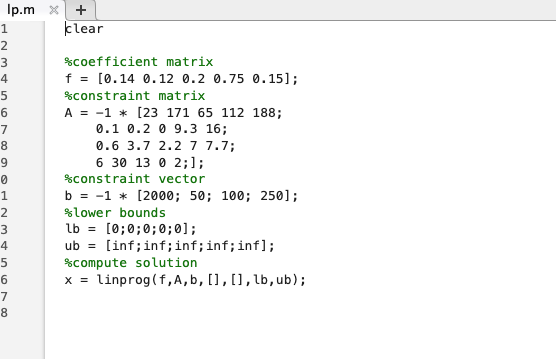
\includegraphics[width=\textwidth]{matlab}
\end{figure}
And I got the following results:
\begin{figure}[H]
\centering
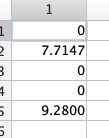
\includegraphics[width=0.2\textwidth]{results}
\end{figure} This tells us that $r = 0$, $b = 7.7147$, $w = 0$, $c = 0$, and $p = 9.28$. That is, we should buy $7.7147$ servings of baked potatoes and $9.28$ servings of peanut butter. The cost of this is 
\[
0.12(7.7147) + 0.15(9.28) = 2.317764
\]
\newpage
\section*{Problem 2}
\subsection*{Part A}
We let $t$ denote Tom's salary, $p$ denote Peter's salary, $n$ denote Nina's salary, $s$ denote Samir's salary, $g$ denote Gary's salary, $l$ denote Linda's salary, and $b$ denote Bob's salary. The first constraint tells us that Tom wants at least $ \$20000$. This informs us that
\[
t \geq 20000
\] The second constraint tells us that Peter, Nina, and Samir each want $\$5000$ more than Tom. Thus, we obtain
\[
p \geq t + 5000,\, n \geq t + 5000,\, s \geq t+ 5000
\] The third constraint tells us that Gary wants his salary to be at least as high as the combined salaries of Tom and Peter. From this, we get
\[
g \geq t + p
\] The fourth constraint tells us that Linda wants to make $\$200$ more than Gary. Thus, we have
\[
l \geq g + 200
\] The fifth condition tells us that the combined salaries of Nina and Samir should be at least twice the combined salary of Tom and Peter. This tells us that
\[
n + s \geq 2(t + p)
\] The next constraint tells us that Bob's salary is at least as high as Peter's and at least as high as Samir's. From this, we obtain
\[
b \geq p,\, b \geq s
\] The seventh condition tells us that the combined salaries of Bob and Peter should be at least $\$60000$. This gives
\[
b + p \geq 60000
\] The eighth condition tells us that Linda should make less money than the combined salaries of Bob and Tom. This gives
\[
l \leq b + t
\] Finally, we must again include the non-negativity constraints. That is, we have
\[
t \geq 0,\, p \geq 0,\, n \geq 0,\, s \geq 0,\, g \geq 0,\, l \geq 0,\, b \geq 0
\] We wish to minimize the following subject to the above constraints:
\[
t+p+n+s+g+l+b
\]
\newpage
\subsection*{Part B}
First, we keep all of the constraints from the previous part. Now, we introduce a new variable $m$. We require
\[
m \geq t,\, m \geq p,\, m\geq n,\, m\geq s,\, m \geq g,\, m \geq l,\, m \geq b
\] Now, the linear program is to minimize $m$ subject to these constraints.
\newpage
\section*{Problem 3}
\subsection*{Part A}
Our goal is to minimize the sum
\[
\sum_{j=1}^q \sum_{i=1}^p c_{ij} x_{ij}
\] First, we note that
\[
x_{ij} \geq 0
\] for all $i,j$. Now, we know that factory $i$ makes $s_i$ units per month and that the stores cannot receive more than $s_i$ units from this factory. Furthermore, the problem tells us that every unit made is shipped to a store. Thus, we may deduce that
\[
x_{i1} + x_{i2} + \cdots + x_{iq} = s_i
\] for every $i$. Furthermore, we know that store $j$ receives $t_j$ units per month from all the factories combined. This tells us that
\[
x_{1j} + x_{2j} + \cdots + x_{pj} = t_j
\] for every $j$. Finally, we should note that $s_i \geq 0$ for all $i$ and that $t_j \geq 0$ for all $j$. These are all the constraints of the linear program. 
\newpage
\subsection*{Part B}
First, we may suppose that the feasible region is nonempty. That is, there exist $x_{ij}$ such that $x_{ij} \geq 0$ and
\[
x_{i1} + x_{i2} + \cdots + x_{iq} = s_i
\] and
\[
x_{1j} + x_{2j} + \cdots + x_{pj} = t_j
\] Summing
\[ 
x_{i1} + x_{i2} + \cdots + x_{iq} = s_i
\] over all $i$ yields
\[
\sum_{j=1}^q \sum_{i=1}^p x_{ij} =  \sum_{i=1}^p s_i
\] Summing 
\[
x_{1j} + x_{2j} + \cdots + x_{pj} = t_j
\] over all $j$ yields
\[
\sum_{j=1}^q \sum_{i=1}^p x_{ij} = \sum_{j=1}^q t_j
\] Thus, we obtain
\[
 \sum_{i=1}^p s_i = \sum_{j=1}^q t_j
\]

Next, we wish to show that if 
\[
\sum_{i=1}^p s_i = \sum_{j=1}^q t_j
\] then the feasible region is nonempty. We induct on the sum $p+q$. For the base case, we suppose that $p+q = 2$. Then, we deduce that $p = q =1$ (since $p$ and $q$ are assumed to be positive integers), and our hypothesis says that
\[
s_1 = t_1
\] Letting $x = s_1 = t_1$, we see that the constraints are all satisfied. Next, we may suppose that $p+q > 2$ and that the result is true for $p+q-1$. Without loss of generality, we may suppose that $s_1 \leq t_1$. We wish to find $x_{ij}$ such that all the constraints are satisfied. Let $x_{11} = s_{1}$ and $x_{1j} = 0$ for all $j \in \{2,\ldots,q\}$. Let $t_1^\prime = t_1 - s_1 \geq 0$. Now, we know that
\[
t_1^\prime + t_2 + \cdots + t_q  = s_2 + \cdots + s_p
\] By our induction hypothesis, we find that there exist $x_{ij}$ with $i \in \{2,\ldots,p\}$ and $j \in \{1,\ldots,q\}$ such that the constraints are satisfied. To be specific, we have
\[
x_{21} + \cdots + x_{p1} = t_1^\prime
\] and
\[
x_{2j} + \cdots + x_{pj} = t_j
\] for all $j \in \{2,\ldots,q\}$ and
\[
x_{i1} + \cdots + x_{iq} = s_i
\] for all $i \in \{2\ldots,p\}$. This almost gives us what we want. Let us consider the equation
\[
x_{21} + \cdots + x_{p1} = t_1^\prime = t_1 - s_1 = t_1 - x_{11}
\] From this, we obtain
\[
x_{11} + x_{21} + \cdots + x_{p1} = t_1
\] Furthermore, we assumed that for every $j \in \{2,\ldots,q\}$, $x_{1j} = 0$. That is, we have
\[
x_{1j} + x_{2j} + \cdots + x_{pj} = t_j
\] Finally, we note that
\[
x_{11} + x_{12} + \cdots + x_{1q} = s_1 + 0 + \cdots + 0 = s_1
\] Thus, we have found a point $\{x_{ij}\}$ in the feasible region, so we know that it is nonempty. I have attached a picture below to make this proof more intuitive. The sum of row $i$ is $s_i$ and the sum of column $j$ is $t_j$.
\begin{figure}[H]
\centering
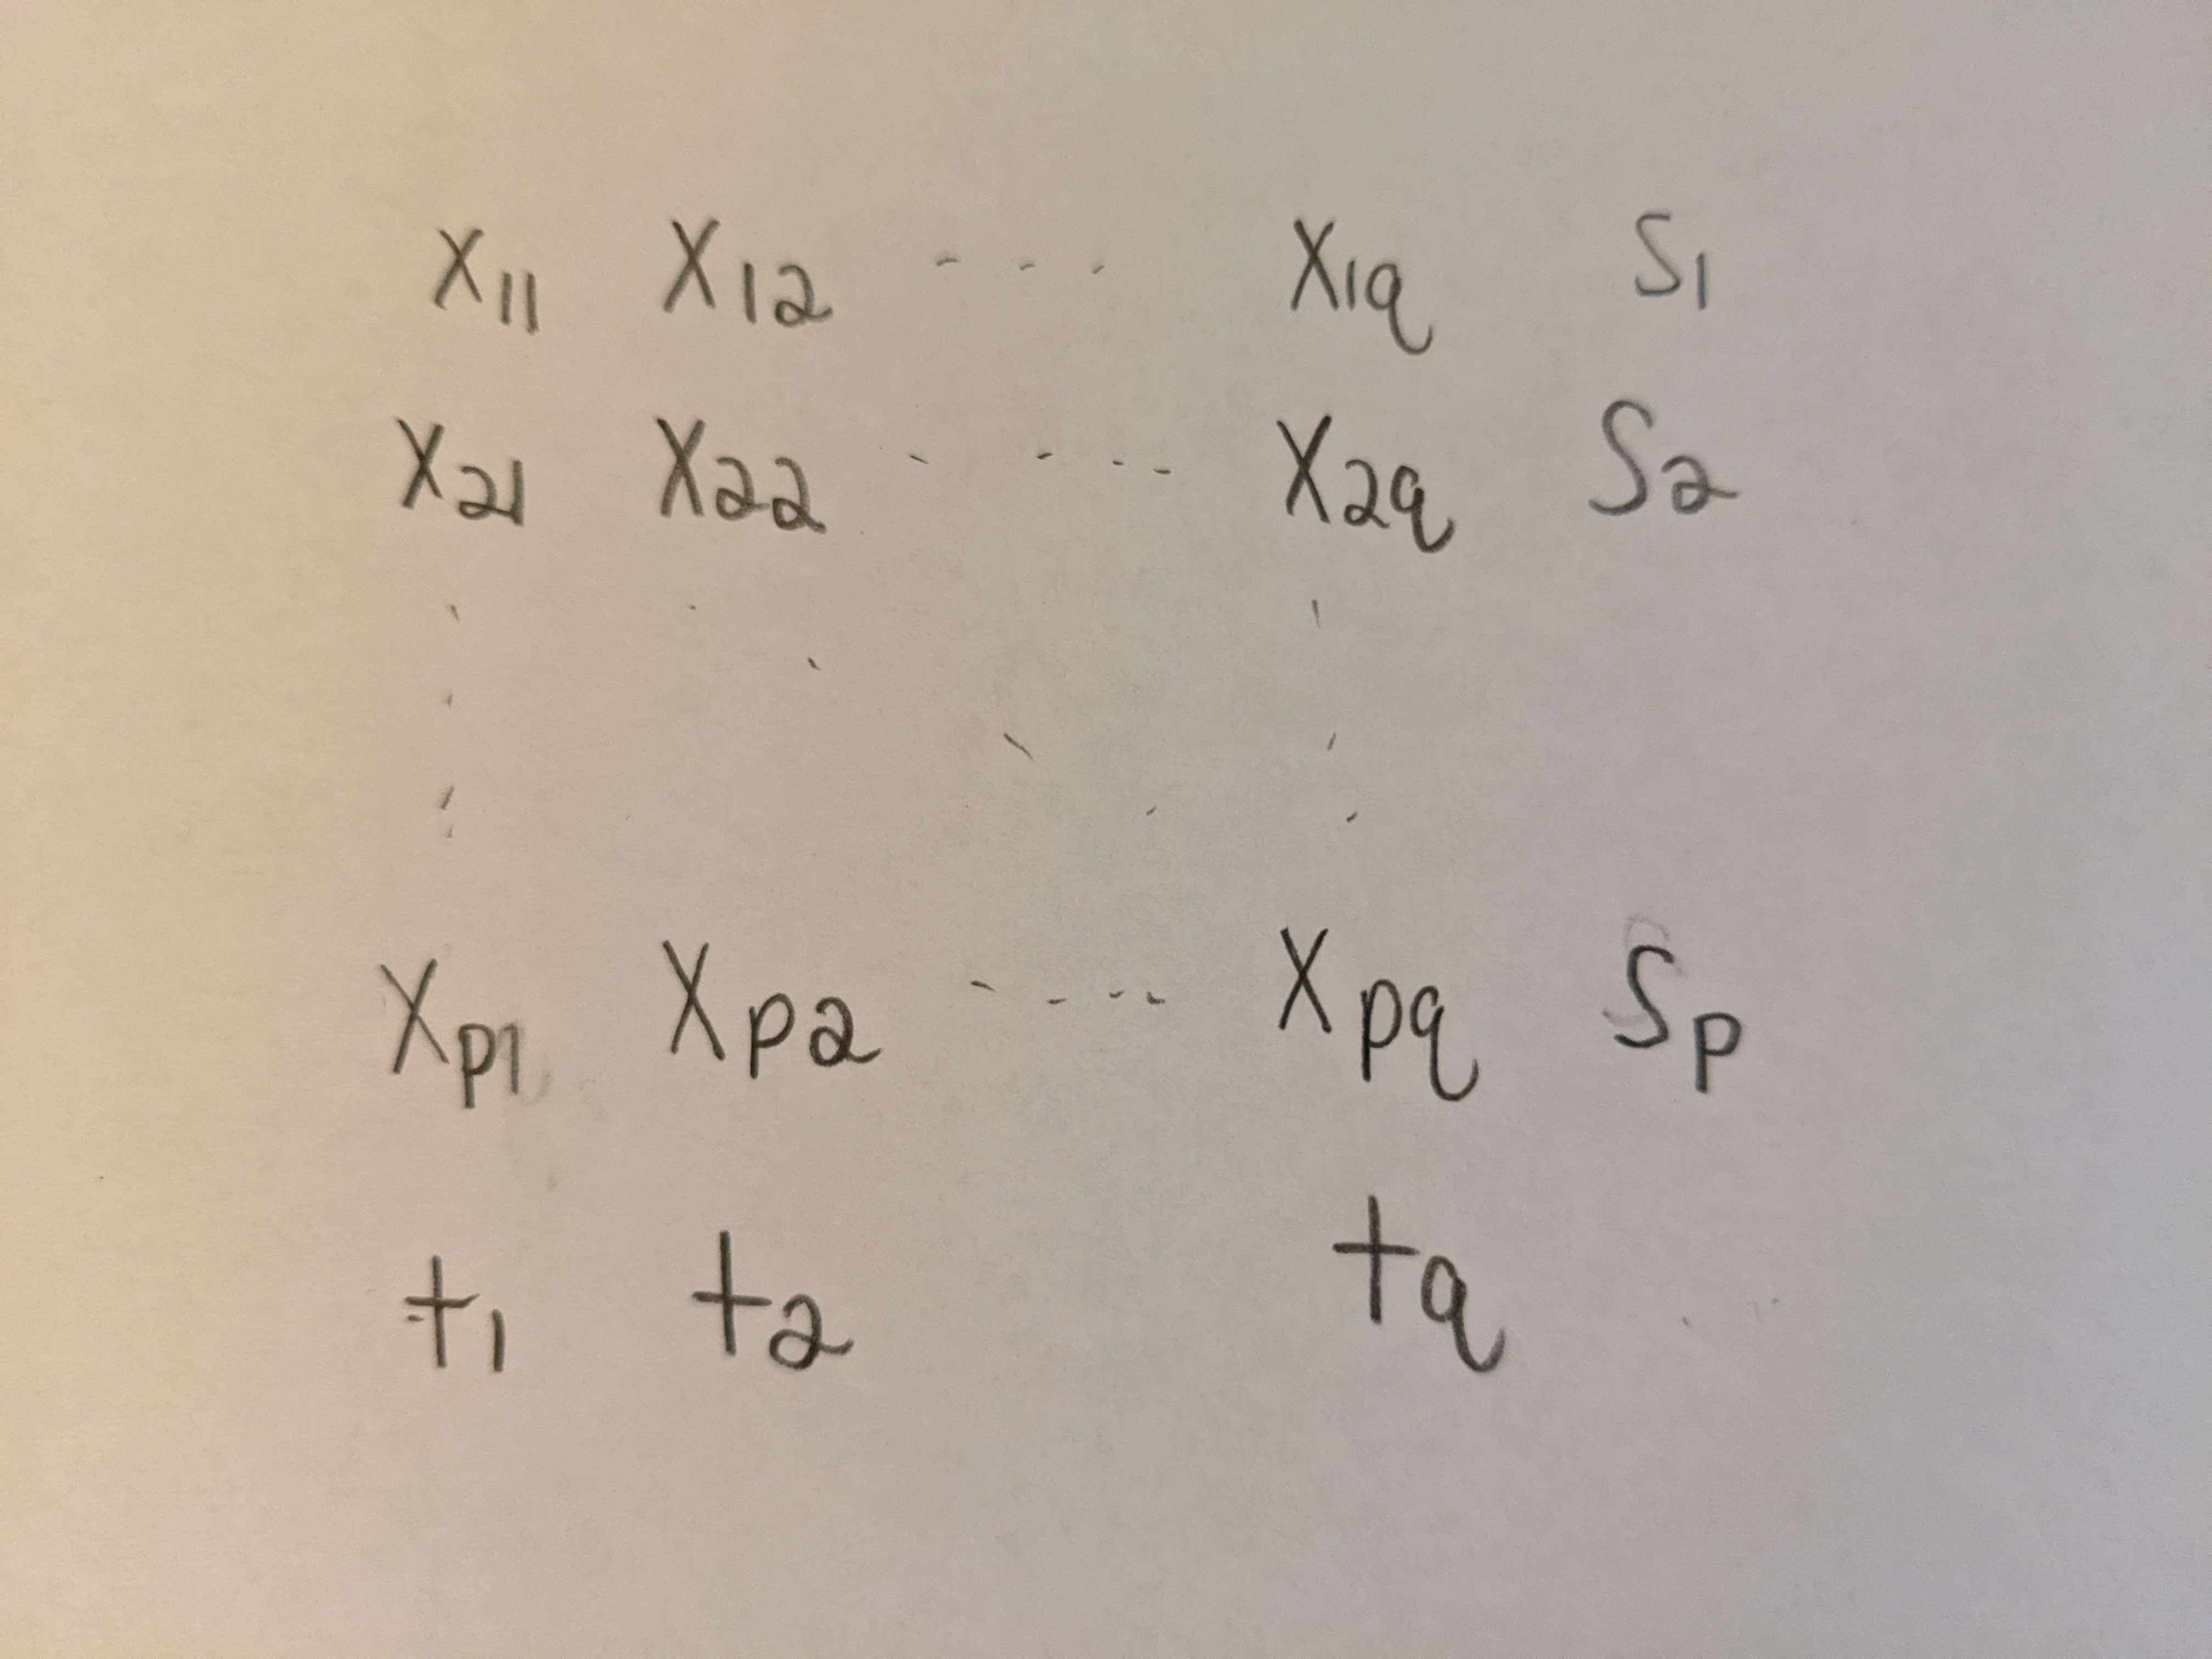
\includegraphics[width=\textwidth]{pic1}
\end{figure}
\newpage
\section*{Problem 4}
\subsection*{Part A}
Let us consider the below picture:
\begin{figure}[H]
\centering
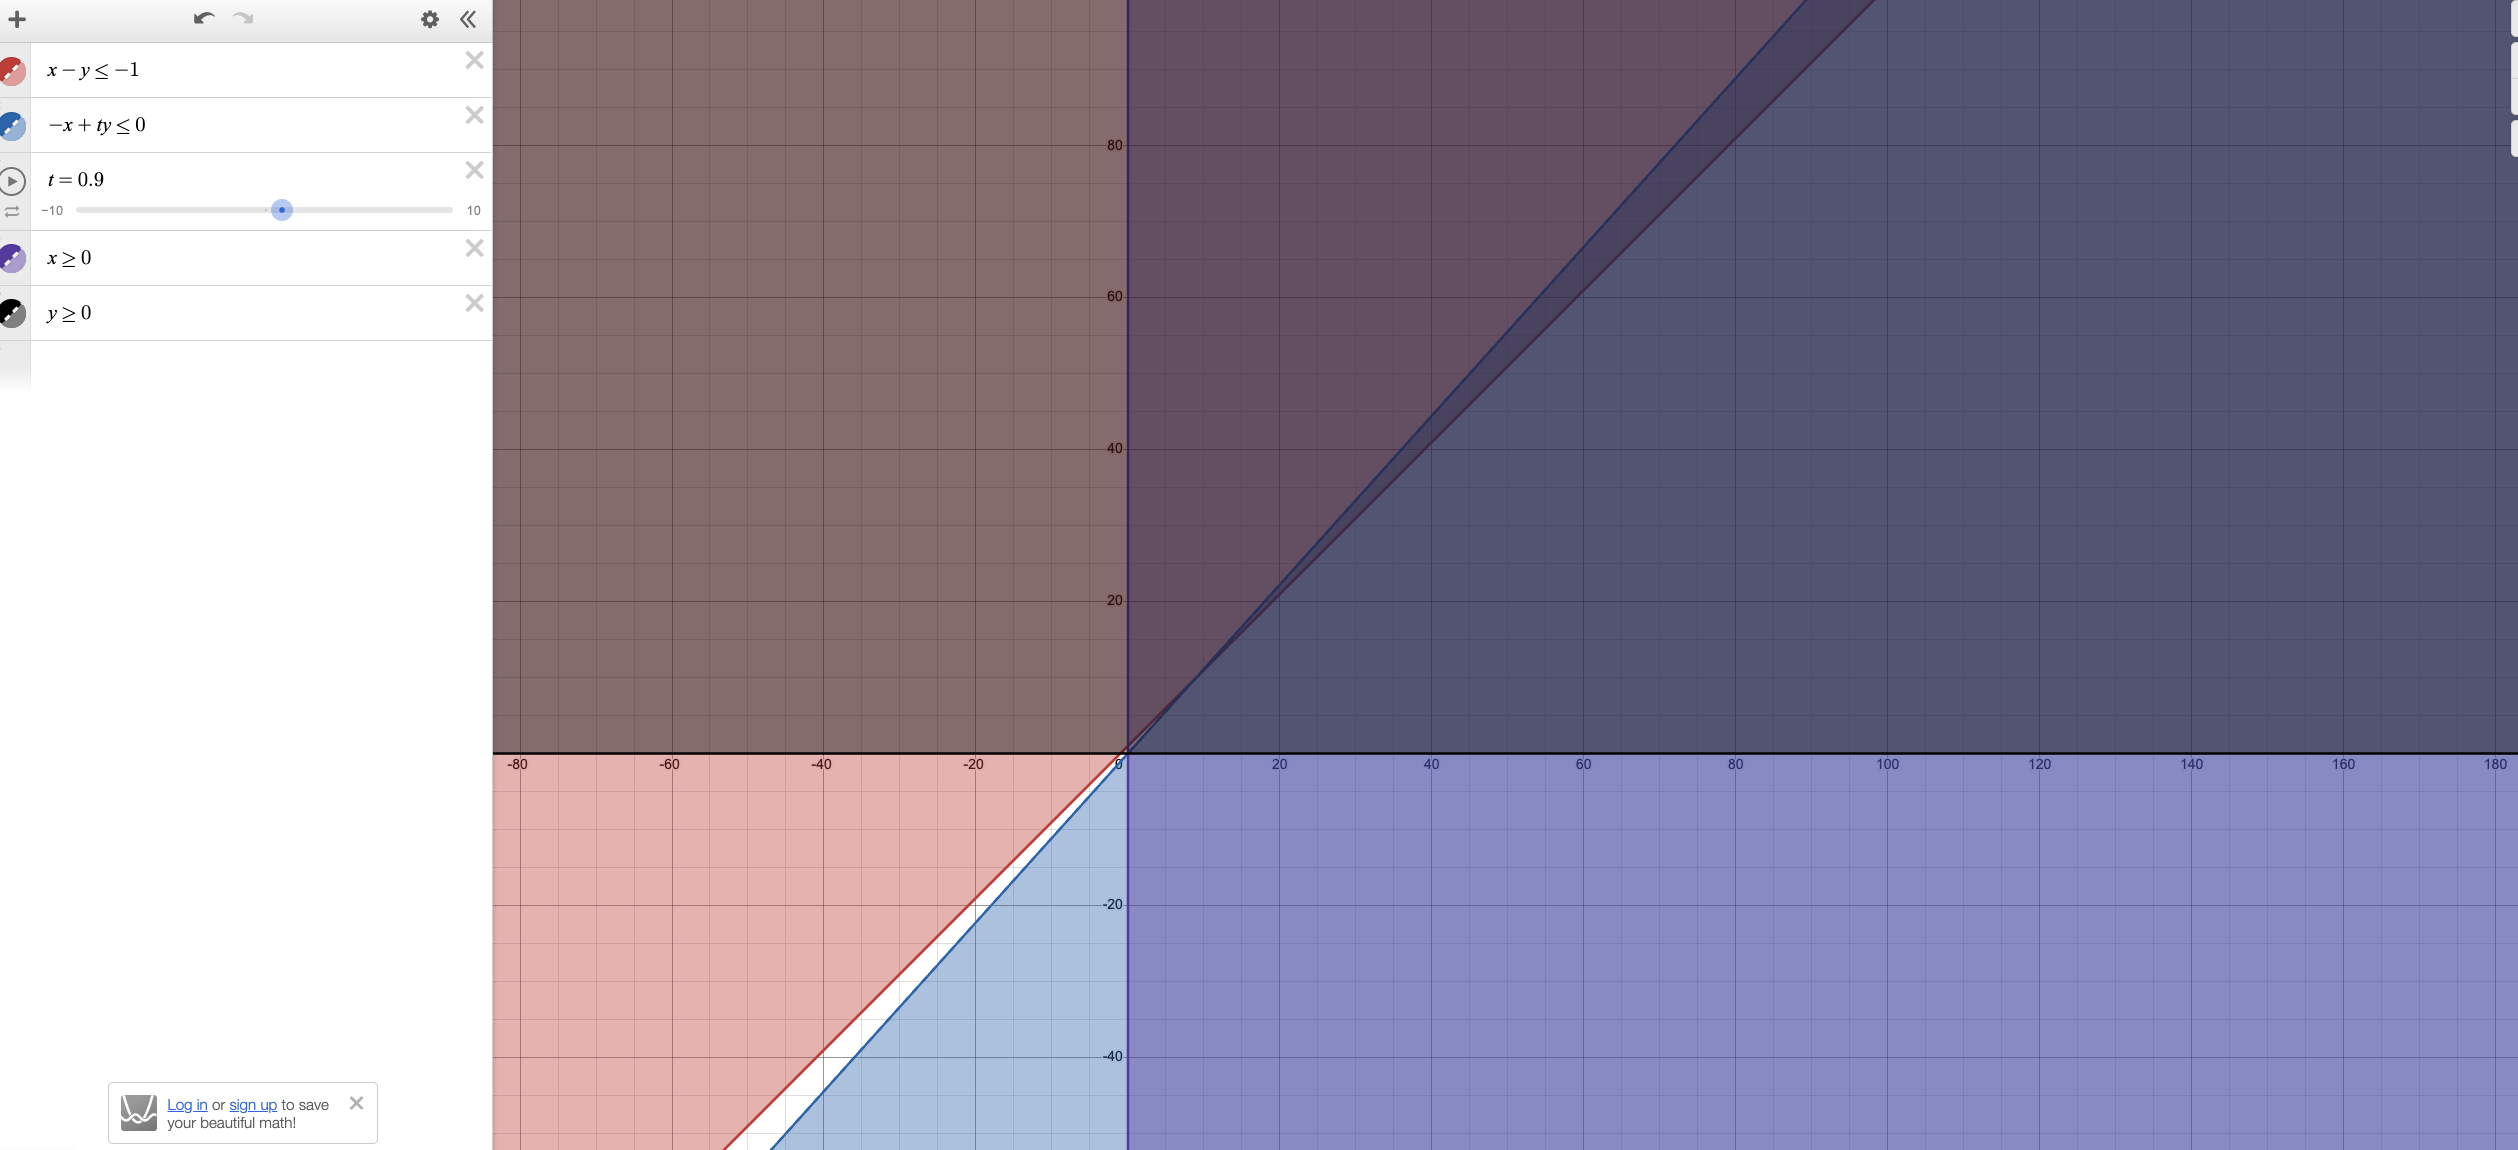
\includegraphics[width=\textwidth]{desmos1}
\end{figure} We wish for all the colored regions to intersect (so that there is a feasible region). This appears to occur when $t < 1$.
\newpage
\subsection*{Part B}
First, we show that if $t < 1$, then there is a feasible region. We consider two cases. First, suppose that $0 \leq t < 1$. In this case, let us solve the system of equations $x_1 - x_2 = -1$ and $-x_1 + tx_2 = 0$. We have $x_1 = -1 + x_2$ so that $1 - x_2 + tx_2 = 0$, which gives us $(t-1)x_2 = -1$. From this, we get 
\[
x_2 = -\frac{1}{t-1} = \frac{1}{1-t} > 0
\] since $1-t > 0$. Now, we have
\[
x_1 = -1 + x_2 = -1 + \frac{1}{1-t} = \frac{t- 1 + 1}{1-t} = \frac{t}{1-t} \geq 0
\] Thus, we have found a point $(x_1,x_2)$ in the feasible region, so the linear program is feasible. Next, we consider the case $t < 0$. Then, we take the point $(0,1)$. Notice that $0-1\leq -1$, that $-0+t \leq 0$, that $0 \geq 0$, and that $1 \geq 0$. Thus $(0,1)$ is a point in the feasible region, so the linear program is feasible.  Next, we show that if the linear program is feasible, then $t$ is in $T = (-\infty,1)$. We show this by contrapositive. That is, we claim that if $t \not \in (-\infty,1)$, the linear program is not feasible. Suppose that $t \geq 1$. First, we consider the specific case $t = 1$. Adding 
\[
x_1-x_2 \leq -1
\] to
\[
-x_1+x_2 \leq 0
\] yields
\[
0 \leq -1
\] a clear contradiction. Next, we suppose that $t > 1$. Then, adding
\[
x_1 - x_2 \leq -1
\] to
\[
-x_1 + tx_2 \leq 0
\] yields
\[
(t-1)x_2 \leq -1
\] or
\[
x_2 \leq \frac{-1}{t-1} < 0
\] again contradicting the constraint that $x_2 \geq 0$. Thus, we find that the linear program is not feasible. This proves that the linear program is feasible if and only if $t \in (-\infty,1)$.
\newpage
\subsection*{Part C}
Consider the below image:
\begin{figure}[H]
\centering
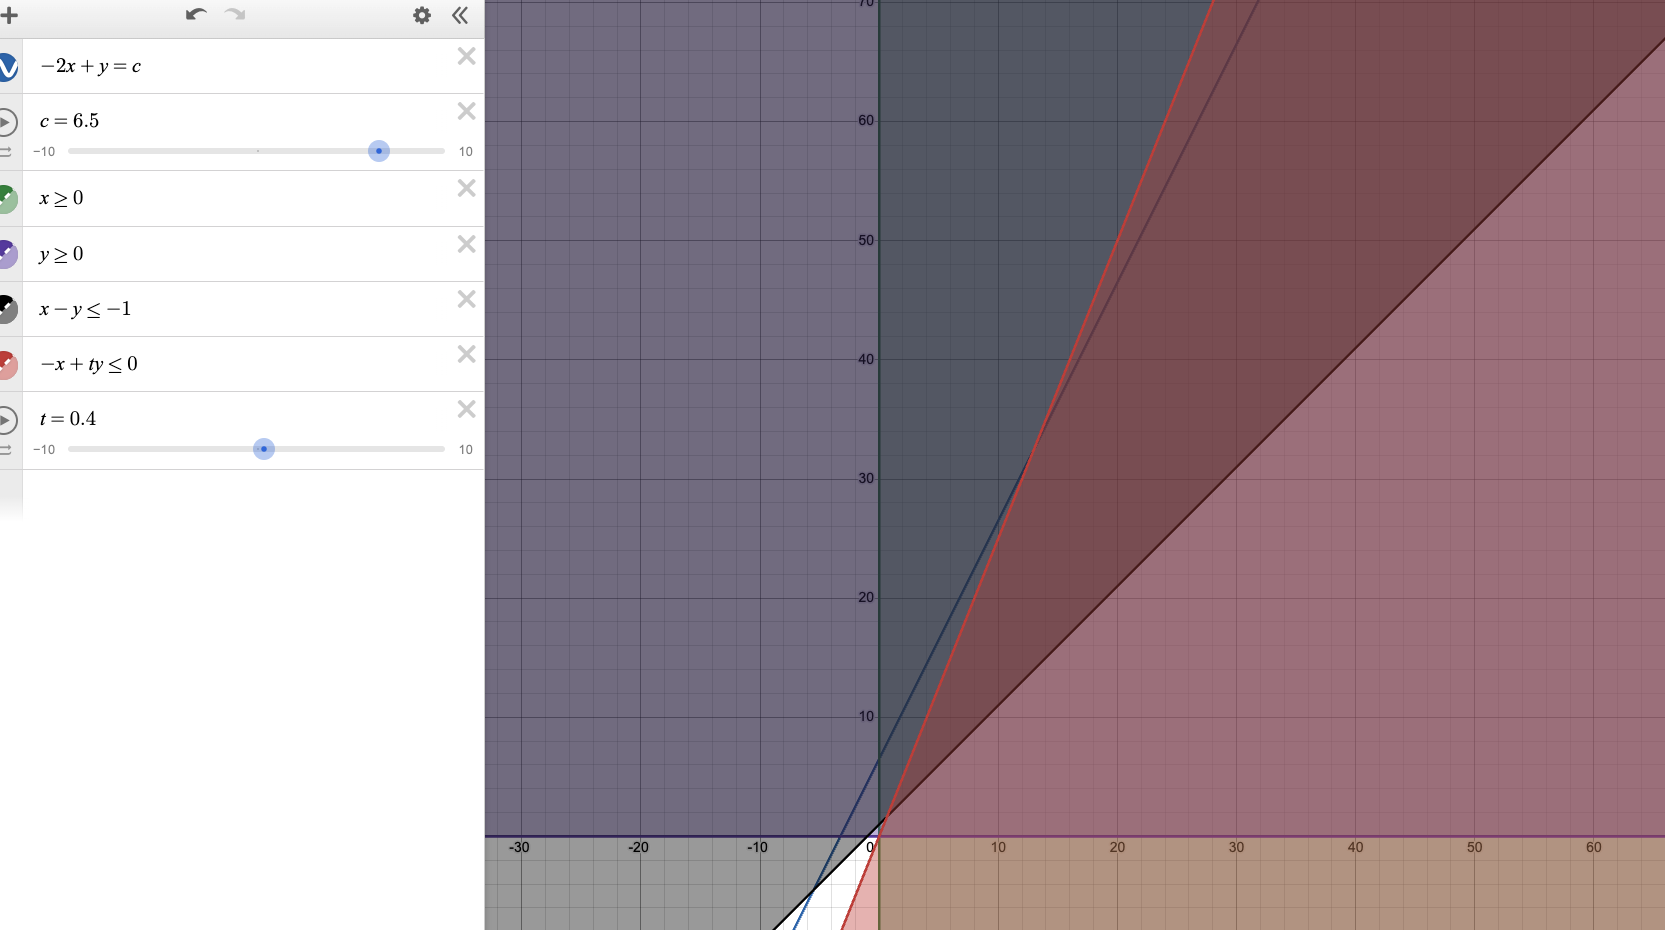
\includegraphics[width=\textwidth]{desmos2}
\end{figure}
We wish for the intersection of the four colored regions to include the line $-2x+y = c$ (for every positive $c$). This seems to occur when $t < \frac{1}{2}$. Thus, we claim that $S = (-\infty,\frac{1}{2})$.
\newpage
\subsection*{Part D}
We wish to show that the linear program is unbounded if and only if $t \in S = (-\infty,\frac{1}{2})$. First, we suppose that $t \in (-\infty,\frac{1}{2})$. Let us consider two cases. First, we suppose that $t\geq 0$. To show that the linear program is unbounded, we let $c > 0$ be an arbitrary positive number. Let us consider the intersection of the lines $-2x_1 + x_2 = c$ and $-x_1 + tx_2 = 0$. First, we note that 
\[
x_1 = tx_2 \implies -2tx_2 + x_2 = c \implies x_2(1-2t) = c \implies x_2 = \frac{c}{1-2t} > 0
\] since we are assuming that $t < 1/2$. This tells us that $x_2$ is positive, which is one of the constraints. Then we get
\[
x_1 = tx_2 = \frac{tc}{1-2t} \geq 0
\] as long as $t \geq 0$ (which we are assuming is true for now). We already know that $-x_1 + tx_2 = 0$, so that constraint is satisfied. The only constraint we have to worry about is
\[
x_1 - x_2 \leq -1
\] Substituting $x_1$ and $x_2$ into this inequality yields
\[
\frac{tc}{1-2t} -  \frac{c}{1-2t} = \frac{c(t-1)}{1-2t} \leq -1
\] Notice that $t-1 < 0$ so that
\[
c \geq \frac{2t-1}{t-1}
\] (the inequality sign is reversed because we are multiplying through by a negative number). So all we have to do is choose $c$ sufficiently large and this inequality is also satisfied. We are allowed to do this because we are attempting to show that the linear program is unbounded above. Next, we consider the case when $t < 0$. In this case, we consider the point $(0,s)$, where $s > 1$. We claim that this point satisfies all the constraints. To do this, we first note that
\[
0\geq 0, s\geq 0
\] so that the nonnegativity constraints are satisfied. Next, we note that
\[
0 - s \leq -1
\] and that
\[
-0 + ts \leq 0
\] because we are assuming that $t <0$ and $s > 1$. Thus, all the constraints are satisfied. Now, we note that
\[
-2x_1 + x_2 = -2(0) + s = s
\] which can be made arbitrarily large simply by increasing $s$. Thus, the linear program is still unbounded.


Next, we must show that if the linear program is unbounded, then $t \in (-\infty, \frac{1}{2})$. We do this by contrapositive. That is, we must show that if $t \not \in (-\infty, \frac{1}{2})$, then the linear program is bounded. In part $B$, we showed that the linear program is not feasible if $t \geq 1$, so we may assume that $t < 1$. To show the linear program is unbounded, we first write
\[
-2x_1 + x_2 = a(x_1-x_2) + b(-x_1 + tx_2) = (a-b)x_1 + (bt - a)x_2
\] This gives us a system of two equations:
\begin{align*}
a-b &= -2\\
bt - a &= 1
\end{align*} Adding them together yields
\[
bt - b = -1 \implies b(t-1) = -1 \implies b = \frac{-1}{t-1} = \frac{1}{1-t}
\] Then we obtain
\[
a-b = -2 \implies a = b-2 = \frac{1}{1-t} - 2 = \frac{1-2(1-t)}{1-t} = \frac{2t -1}{1-t}
\] so we get
\[
-2x_1 + x_2 =  \frac{2t -1}{1-t}(x_1-x_2) + \frac{1}{1-t}(-x_1 + tx_2)
\] Because we are assuming that $\frac{1}{2} \leq t < 1$, we obtain
\[
\frac{2t-1}{1-t} \geq 0,\, \frac{1}{1-t} > 0
\] This ensures that we don't have to flip the signs of the following inequalites:
\begin{align*}
x_1 - x_2 &\leq -1\\
-x_1 + tx_2 &\leq 0
\end{align*} Now we find that
\[
-2x_1 + x_2 =  \frac{2t -1}{1-t}(x_1-x_2) + \frac{1}{1-t}(-x_1 + tx_2) \leq \frac{1-2t}{1-t}
\] so the linear program is bounded. Thus we find that the linear program is unbounded if and only if $t \in (-\infty,\frac{1}{2})$.
\end{document} 